\documentclass[a4paper]{article}
\usepackage[utf8]{vietnam}
\usepackage[left=3cm,right=2cm,top=2cm,bottom=2cm]{geometry}
\usepackage{amsmath}
\setlength{\parindent}{0pt}
\usepackage{graphicx} 
\usepackage{multirow}
\usepackage{url}
%\usepackage{wallpaper}
%\usepackage[firstpage]{draftwatermark} 
\usepackage{xcolor}
\usepackage{tikz} 
\usepackage{scrextend}
\usepackage{ulem}
\changefontsizes{13pt}
%\usepackage{background}
\usetikzlibrary{calc}
\usepackage{fancyhdr}
\usepackage[sorting=none]{biblatex}
\addbibresource{references.bib}

\usepackage{titlesec}
\usepackage{enumitem}
\usepackage{amsmath}
\titleformat{\section}{\fontsize{13}{15}\selectfont\bfseries}{\thesection}{1em}{}
\titleformat{\subsection}{\fontsize{13}{15}\selectfont\bfseries}{\thesubsection}{1em}{}
\usepackage{enumitem}
%----------------------- config của sy-------------
\usepackage{setspace}
\onehalfspacing
\usepackage{float}
\restylefloat{figure}
\floatplacement{figure}{H}
\usepackage{indentfirst}
\setlength{\parindent}{1cm}
%--------------------------------------Header footer------------------------------------
\pagestyle{fancy}
\fancyhf{} % Xóa định dạng hiện tại của header và footer

% Header
\lhead{Nhóm 4}
\chead{}
\rhead{Học phần: Mạng định nghĩa bằng phần mềm}

% Footer
\lfoot{}
\cfoot{} % Hiển thị số trang ở giữa footer
\rfoot{\thepage}

% Định dạng các đường line ở header và footer
\renewcommand{\headrulewidth}{0.1pt} % Độ dày của đường line ở header
\renewcommand{\footrulewidth}{0.1pt} % Độ dày của đường line ở footer
%---------------------------------------------------------------------------------------
%\backgroundsetup{scale = 1, angle = 0, opacity = 0.2,
%contents = {\includegraphics[width = 0.9\paperwidth,
%height = 0.9\paperheight, keepaspectratio] {hust.png}}}

%\backgroundsetup{scale = 1, angle = 0, opacity = 0.2,
%contents = {\includegraphics[width = 0.97\paperwidth,
%height = 0.97\paperheight, keepaspectratio] {bia.png}}}
\begin{document}

\begin{titlepage}
%\SetWatermarkText{\includegraphics[width = 0.97\paperwidth,
%height = 0.97\paperheight]{bia.png}}
%\SetWatermarkAngle{0} 
%\SetWatermarkText{\includegraphics[scale=1]{hust.png}}
%\SetWatermarkAngle{0} 
\begin{tikzpicture}[remember picture,overlay,inner sep=0,outer sep=0]
     \draw[black!80!black,line width=4pt] ([xshift=-2cm,yshift=-2cm]current page.north east) coordinate (A)--([xshift=3cm,yshift=-2cm]current page.north west) coordinate(B)--([xshift=3cm,yshift=2cm]current page.south west) coordinate (C)--([xshift=-2cm,yshift=2cm]current page.south east) coordinate(D)--cycle;

     \draw ([yshift=0.5cm,xshift=-0.5cm]A)-- ([yshift=0.5cm,xshift=0.5cm]B)--
     ([yshift=-0.5cm,xshift=0.5cm]B) --([yshift=-0.5cm,xshift=-0.5cm]B)--([yshift=0.5cm,xshift=-0.5cm]C)--([yshift=0.5cm,xshift=0.5cm]C)--([yshift=-0.5cm,xshift=0.5cm]C)-- ([yshift=-0.5cm,xshift=-0.5cm]D)--([yshift=0.5cm,xshift=-0.5cm]D)--([yshift=0.5cm,xshift=0.5cm]D)--([yshift=-0.5cm,xshift=0.5cm]A)--([yshift=-0.5cm,xshift=-0.5cm]A)--([yshift=0.5cm,xshift=-0.5cm]A);

     \draw ([yshift=-0.3cm,xshift=0.3cm]A)-- ([yshift=-0.3cm,xshift=-0.3cm]B)--
     ([yshift=0.3cm,xshift=-0.3cm]B) --([yshift=0.3cm,xshift=0.3cm]B)--([yshift=-0.3cm,xshift=0.3cm]C)--([yshift=-0.3cm,xshift=-0.3cm]C)--([yshift=0.3cm,xshift=-0.3cm]C)-- ([yshift=0.3cm,xshift=0.3cm]D)--([yshift=-0.3cm,xshift=0.3cm]D)--([yshift=-0.3cm,xshift=-0.3cm]D)--([yshift=0.3cm,xshift=-0.3cm]A)--([yshift=0.3cm,xshift=0.3cm]A)--([yshift=-0.3cm,xshift=0.3cm]A);

   \end{tikzpicture}


\begin{center}
    \vspace{7pt}
    \fontsize{14pt}{16pt}
    \textbf{TRƯỜNG ĐẠI HỌC BÁCH KHOA - ĐẠI HỌC ĐÀ NẴNG}
    
    \vspace{7pt}
    \textbf{KHOA ĐIỆN TỬ - VIỄN THÔNG} \\
    **************************
\end{center}
\vspace{10pt}
\begin{center}
    \includegraphics[scale=0.37]{images/logodut.jpg}
    \includegraphics[scale=0.75]{images/logoete.jpg}
    
    \vspace{20pt}
    \fontsize{17pt}{17pt}\selectfont 
    \textbf{BÁO CÁO CUỐI KỲ} \\
    \vspace{7pt}
    \textbf{Học phần: Mạng định nghĩa bằng phần mềm}
    \vspace{7pt}

\end{center}
\begin{flushleft}
    \fontsize{15pt}{10pt}\selectfont  
    \textbf{\textsl{\hspace{27pt}{\uline{ĐỀ TÀI:}}}}
\end{flushleft}
\begin{center}
    \hspace{10pt}
    \fontsize{16pt}{16pt}\selectfont 
    \textbf{\textrm{Phát hiện và giảm thiểu tấn công DDoS bằng \\ Machine Learning trong SDN}}
\end{center}
\begin{center}
    \fontsize{16pt}{17pt}\selectfont 
    \textbf{\textrm{}}
\end{center}

\vspace{50pt}
\begin{addmargin}[1cm]{0cm}
\textbf{Giảng viên hướng dẫn: \hspace{2cm}TS. Tăng Anh Tuấn}
\end{addmargin}
\vspace{10pt}
% Bảng sinh viên thực hiện thụt vào 2cm
\begin{addmargin}[1cm]{0cm}
\textbf{Sinh viên thực hiện: \hspace{2.6cm}Nhóm 4}
\begin{tabbing}
\hspace{6cm}\=\hspace{3cm}\=\hspace{5cm} \kill
{\textbf{Họ và tên}}\>{\textbf{MSSV}}\>{\textbf{Lớp học phần}}\\
\hspace{6cm}\=\hspace{3cm}\=\hspace{5cm} \kill
Lê Phạm Công\> 106200221\> 20.44\\
\hspace{6cm}\=\hspace{3cm}\=\hspace{5cm} \kill
Phan Công Danh\> 106200222\> 20.44\\

\end{tabbing}
\end{addmargin}
\vspace{1cm}
\begin{center}
    \textit{\textbf{Đà Nẵng, ngày 17 tháng 05 năm 2024}}
\end{center}
\end{titlepage}
% -------------------------------------End trang bìa-----------------------
\newpage
\tableofcontents
\newpage

% ----------------------- MAIN DOCUMENT---------------------------%

\section*{Tóm tắt}
\addcontentsline{toc}{section}{Tóm tắt}
Tấn công DDoS (Distributed Denial of Service- Tấn công từ chối dịch vụ phân tán) là một trong những mối đe dọa nghiêm trọng nhất đối với an ninh mạng hiện nay. Chúng có khả năng gây ra sự gián đoạn nghiêm trọng cho các dịch vụ và ứng dụng quan trọng bằng cách tràn ngập hệ thống mục tiêu với lưu lượng truy cập khổng lồ, vượt quá khả năng xử lý của nó. Với sự phát triển của công nghệ mạng và sự gia tăng số lượng thiết bị IoT, các cuộc tấn công DDoS ngày càng trở nên phức tạp và mạnh mẽ hơn, làm tăng nhu cầu về các giải pháp hiệu quả để phát hiện và giảm thiểu chúng.

Báo cáo này tập trung khai thác tiềm năng của Machine Learning (ML) để phát hiện các cuộc tấn công DDoS trong môi trường mạng SDN (Software-Defined Networking).  Mục tiêu của đồ án là xây dựng được hệ thống SDN, mô phỏng các cuộc tấn công DDOS và thử nghiệm các phương pháp phát hiện và giảm thiểu. Kết quả thực nghiệm cho thấy phương pháp phát hiện và giảm thiểu tấn công DDoS dựa trên Machine Learning kết hợp được đề xuất có tỷ lệ phát hiện tốt đối với tấn công DDoS phổ biến.

Mã nguồn của báo cáo có thể được tìm thấy tại: \url{https://github.com/lephamcong/DDoS_Detection_and_Mitigation_in_SDN.git}

\section{Giới thiệu}
Với sự phát triển không ngừng của công nghệ mạng, sự gia tăng liên tục của nhu cầu kinh doanh trực tuyến và sự bùng nổ của nền kinh tế Internet trong kỷ nguyên số, các dịch vụ mạng chứa thông tin quan trọng về kinh doanh và ngành công nghiệp đã trở thành một phần không thể thiếu trong sản xuất và đời sống xã hội hiện nay. Sự xuất hiện của các cuộc tấn công DDoS có thể gây ra sự gián đoạn nghiêm trọng cho các dịch vụ mạng liên quan, dẫn đến tổn thất kinh tế lớn và thậm chí có thể gây ra những hậu quả thảm khốc khác. Các cuộc tấn công DDoS là một trong những mối đe dọa nghiêm trọng nhất đối với an ninh mạng mà Internet phải đối mặt. Phát hiện chính xác và nhanh chóng các cuộc tấn công DDoS là một chủ đề nghiên cứu trọng yếu trong lĩnh vực an ninh mạng. Mạng được định nghĩa bằng phần mềm (SDN) là một kiến trúc mới nổi, năng động, dễ quản lý, tiết kiệm chi phí và có khả năng thích ứng, khiến nó trở nên lý tưởng cho tính chất năng động, băng thông cao của các ứng dụng ngày nay. Kiến trúc này tách riêng các chức năng điều khiển và chuyển tiếp mạng cho phép điều khiển mạng trở nên có thể lập trình trực tiếp và cơ sở hạ tầng cơ bản được trừu tượng hóa cho các ứng dụng và dịch vụ mạng. 

Trong kiến trúc mạng truyền thống, các phương pháp chính của công nghệ phát hiện tấn công DDoS có thể được chia thành phát hiện tấn công dựa trên đặc điểm lưu lượng và phát hiện tấn công dựa trên bất thường lưu lượng. Phương pháp đầu tiên chủ yếu thu thập tất cả các thông tin đặc điểm liên quan đến cuộc tấn công và thiết lập cơ sở dữ liệu đặc điểm của tấn công DDoS. Bằng cách so sánh và phân tích thông tin dữ liệu của gói dữ liệu mạng hiện tại với cơ sở dữ liệu đặc điểm, chúng ta có thể xác định liệu có bị tấn công DDoS hay không. Các phương pháp thực hiện chính bao gồm so khớp đặc điểm, suy luận mô hình, chuyển trạng thái và hệ chuyên gia. Phương pháp thứ hai chủ yếu là thiết lập mô hình lưu lượng và phân tích các thay đổi lưu lượng bất thường để xác định xem lưu lượng có bất thường hay không, từ đó phát hiện liệu máy chủ có bị tấn công hay không.

Trong mạng SDN (Software Defined Networking), phát hiện các cuộc tấn công DDoS được thực hiện hiệu quả nhờ vào tính linh hoạt và quản lý tập trung của SDN. Các phương pháp chính bao gồm phân tích lưu lượng dựa trên dữ liệu lớn, sử dụng các công cụ để thu thập và phân tích lưu lượng mạng trong thời gian thực. Học máy (Machine Learning) áp dụng các thuật toán như SVM, Decision Tree, Random Forest và Deep Learning để tự động phát hiện các mẫu bất thường. Phân tích hành vi (Behavioral Analysis) và giám sát luồng (Flow Monitoring) sử dụng các công cụ như Snort và OpenFlow để phát hiện các dấu hiệu tấn công. Phát hiện dựa trên ngưỡng (Threshold-based Detection\cite{halman2024threshold}) cảnh báo khi lưu lượng vượt ngưỡng thiết lập, trong khi các hệ thống cảnh báo sớm (Early Warning Systems) giúp nhận diện dấu hiệu tấn công sớm. Nhờ khả năng lập trình và quản lý tập trung của SDN, các phương pháp này có thể kết hợp để phát hiện và ngăn chặn hiệu quả các cuộc tấn công DDoS, bảo vệ dịch vụ mạng trong môi trường SDN.

Báo cáo này áp dụng Machine Learning để phát hiện cuộc tấn công DDoS và thực hiện biện pháp giảm thiểu nhằm bảo vệ hệ thống mạng. Các đặc trưng của lưu lượng truy cập bình thường và lưu lượng truy cập trong trường hợp giả định là một cuộc tấn công DDoS sẽ được thu thập làm dữ liệu cho bộ phân loại dựa trên thuật toán Machine Learning, từ đó có thể xác định được đâu là một cuộc tấn công DDoS.

\newpage
\section{Cơ sở lý thuyết}
\subsection{Mạng định nghĩa bằng phần mềm (Software Defined Network- SDN)}
Mạng được định nghĩa bằng phần mềm (SDN) là một kiến trúc mới nổi, năng động, dễ quản lý, tiết kiệm chi phí và có khả năng thích ứng, khiến nó trở nên lý tưởng cho tính chất năng động, băng thông cao của các ứng dụng ngày nay. Kiến trúc này tách riêng các chức năng điều khiển và chuyển tiếp mạng cho phép điều khiển mạng trở nên có thể lập trình trực tiếp và cơ sở hạ tầng cơ bản được trừu tượng hóa cho các ứng dụng và dịch vụ mạng.
Mạng SDN cho phép quản trị viên kiểm soát lưu lượng truy cập từ bảng điều khiển trung tâm mà không cần chú ý đến các switch trong mạng. Bộ điều khiển SDN tập trung chỉ đạo các thiết bị chuyển mạch cung cấp các dịch vụ mạng khi cần thiết, với tất cả các kết nối giữa máy chủ và thiết bị.

\begin{figure}
    \centering
    \includegraphics[width=0.7\linewidth]{images/sdn.png}
    \caption{Kiến trúc mạng định nghĩa bằng phần mềm}
    \label{fig:sdn}
\end{figure}
Kiến trúc của SDN bao gồm 3 lớp: lớp ứng dụng (Application Plane), lớp điều khiển (Control Plane) và lớp cơ sở hạ tầng (Data Plane) được thể hiện như hình \ref{fig:sdn}.

Trong một mạng truyền thống, mỗi switch đều có một lớp dữ liệu (data plane) riêng cũng như lớp điều khiển (control plane) riêng. Lớp điều khiển của các switch khác nhau trao đổi thông tin cấu trúc mạng và từ đó xây dựng một bảng chuyển tiếp (forwarding table) quyết định nơi mà một gói dữ liệu đầu vào phải được chuyển tiếp thông qua lớp dữ liệu. Mạng được định nghĩa bằng phần mềm (SDN) là một phương pháp mà chúng ta lấy lớp điều khiển ra khỏi switch và gán nó cho một đơn vị tập trung gọi là bộ điều khiển SDN (SDN controller). Do đó, một quản trị mạng có thể điều chỉnh lưu lượng thông qua một bảng điều khiển tập trung mà không cần phải chạm vào các switch cá nhân. Lớp dữ liệu vẫn nằm trong switch và khi một gói tin đi vào switch, hoạt động chuyển tiếp của nó được quyết định dựa trên các mục nhập trong bảng luồng (flow table), mà được điều chỉnh trước bởi bộ điều khiển. Một bảng luồng bao gồm các trường khớp (như số cổng đầu vào và header gói tin) và hướng dẫn. Gói tin được khớp đầu tiên với các trường khớp của các mục nhập trong bảng luồng. Sau đó, các hướng dẫn của mục nhập luồng tương ứng được thực thi. Các hướng dẫn có thể là chuyển tiếp gói tin qua một hoặc nhiều cổng, loại bỏ gói tin, hoặc thêm tiêu đề vào gói tin. Nếu một gói tin không tìm thấy một trường khớp tương ứng trong bảng luồng, switch sẽ truy vấn bộ điều khiển, bộ điều khiển sẽ gửi một mục luồng mới đến switch. Switch chuyển tiếp hoặc loại bỏ gói tin dựa trên mục luồng này\cite{geeksforgeeks_sdn}.

Một kiến trúc SDN điển hình bao gồm ba lớp:
\begin{itemize}
    \item Lớp ứng dụng (Application Layer): Nó chứa các ứng dụng mạng điển hình như phát hiện xâm nhập, tường lửa và cân bằng tải.
    \item Lớp điều khiển (Control Layer): Nó bao gồm bộ điều khiển SDN, được xem như bộ não của mạng. Nó cũng cho phép trừu tượng phần cứng đối với các ứng dụng được viết trên đầu của nó.
    \item Lớp cơ sở hạ tầng (Infrastructure Layer): Lớp này bao gồm các switch vật lý tạo thành lớp dữ liệu và thực hiện việc chuyển động thực sự của các gói dữ liệu.
\end{itemize}
Các lớp giao tiếp thông qua một tập hợp các giao diện được gọi là northbound APIs và southbound APIs.
Một số mô hình khác nhau của SDN\cite{geeksforgeeks_sdn}:
\begin{itemize}
    \item Open SDN (hình \ref{fig:openSDN}): được triển khai bằng cách sử dụng switch OpenFlow. Đây là một cách triển khai đơn giản của SDN. Trong Open SDN, bộ điều khiển giao tiếp với các switch bằng cách sử dụng southbound APIs thông qua giao thức OpenFlow.
    \begin{figure}
        \centering
        \includegraphics[width=0.35\linewidth]{images/openSDN.png}
        \caption{openSDN}
        \label{fig:openSDN}
    \end{figure}
    \item SDN via APIs: các chức năng trong các thiết bị từ xa như switch được gọi bằng các phương pháp truyền thống như SNMP hoặc CLI hoặc thông qua các phương pháp mới như Rest API. Ở đây, các thiết bị được cung cấp với điểm điều khiển cho phép bộ điều khiển thao tác các thiết bị từ xa bằng cách sử dụng các API.
    \item SDN via Hypervisor-based Overlay Network (hình \ref{fig:Hypervisor-based}): cấu hình của các thiết bị vật lý không thay đổi. Thay vào đó, các mạng lớp phủ dựa trên Hypervisor được tạo ra trên mạng vật lý. Chỉ có các thiết bị ở biên của mạng vật lý được kết nối với các mạng ảo hóa, do đó che giấu thông tin của các thiết bị khác trong mạng vật lý.
    \begin{figure}
        \centering
        \includegraphics[width=0.4\linewidth]{SDN via Hypervisor-based Overlay Network.png}
        \caption{SDN via Hypervisor-based Overlay Network}
        \label{fig:Hypervisor-based}
    \end{figure}
    \item Hybrid SDN là sự kết hợp của Mạng truyền thống với Mạng được định nghĩa bằng phần mềm trong một mạng duy nhất để hỗ trợ các loại chức năng khác nhau trên một mạng.
\end{itemize}
Bảng \ref{tab:sdn_vs_traditional} so sánh một số điểm khác nhau giữa Mạng định nghĩa bằng phần mềm và Mạng truyền thống.
\begin{table}[htbp]
    \centering
    \caption{So sánh giữa Mạng Định Nghĩa Bằng Phần Mềm và Mạng Truyền Thống}
    \label{tab:sdn_vs_traditional}
    \addvspace{0.3cm} % Thêm khoảng cách 0.3cm giữa tên bảng và bảng
    \begin{tabular}{|p{7cm}|p{7cm}|}
        \hline
        \multicolumn{1}{|c|}{\textbf{Mạng Định Nghĩa Bằng Phần Mềm}} & \multicolumn{1}{c|}{\textbf{Mạng Truyền Thống}} \\
        \hline
        Mạng Định Nghĩa Bằng Phần Mềm là một cách tiếp cận mạng ảo. & Mạng truyền thống là cách tiếp cận mạng cổ điển. \\
        \hline
        Kiểm soát tập trung. & Kiểm soát phân tán. \\
        \hline
        Có thể lập trình được. & Không thể lập trình được. \\
        \hline
        Có giao diện mở. & Có giao diện đóng. \\
        \hline
        Data plane và Control Plane được tách biệt bởi phần mềm. & Data Plane và Control Plane được gắn kết trên cùng một mặt phẳng. \\
        \hline
    \end{tabular}
\end{table}

\textbf{Ưu điểm của SDN (Software-Defined Networking):}
\begin{itemize}
    \item \textbf{Tập trung quản lý và kiểm soát mạng}: SDN tách biệt phần điều khiển mạng (\textit{control plane}) khỏi phần chuyển tiếp dữ liệu (\textit{data plane}), cho phép quản lý và kiểm soát toàn bộ mạng từ một điểm trung tâm duy nhất.
    \item \textbf{Khả năng lập trình cao}: Với việc tách biệt phần điều khiển, SDN cung cấp khả năng lập trình mạng, giúp quản lý và cấu hình mạng một cách linh hoạt và hiệu quả hơn.
    \item \textbf{Ảo hóa mạng}: SDN cho phép ảo hóa tài nguyên mạng vật lý, tạo ra các mạng ảo riêng biệt cho các ứng dụng và dịch vụ khác nhau, tăng cường hiệu quả sử dụng tài nguyên.
    \item \textbf{Đổi mới và triển khai nhanh}: Nhờ khả năng lập trình, SDN giúp đơn giản hóa việc triển khai và đổi mới các tính năng mạng mới, giảm thời gian và chi phí.
    \item \textbf{Hỗ trợ điện toán đám mây}: SDN là một công nghệ quan trọng trong việc hỗ trợ và cải thiện các dịch vụ điện toán đám mây, cho phép quản lý tài nguyên mạng một cách hiệu quả hơn.
    \item \textbf{An ninh mạng tăng cường}: Với khả năng giám sát và kiểm soát tập trung, SDN có thể được sử dụng để triển khai các giải pháp an ninh mạng hiệu quả hơn.
\end{itemize}

\textbf{Nhược điểm của SDN:}
\begin{itemize}
    \item \textbf{Phụ thuộc vào bộ điều khiển trung tâm}: SDN phụ thuộc vào bộ điều khiển trung tâm để quản lý và kiểm soát mạng. Nếu bộ điều khiển bị lỗi hoặc tấn công, toàn bộ mạng sẽ bị ảnh hưởng.
    \item \textbf{Vấn đề tương thích và di chuyển}: Việc chuyển đổi từ mạng truyền thống sang SDN có thể gặp phải vấn đề tương thích và khó khăn trong di chuyển.
    \item \textbf{Yêu cầu về nhân lực có kỹ năng chuyên môn}: Triển khai và vận hành SDN đòi hỏi nhân lực có kỹ năng chuyên môn cao về lập trình mạng và quản lý hệ thống phức tạp.
    \item \textbf{Rủi ro về bảo mật}: Tập trung điều khiển mạng tại một điểm duy nhất cũng làm tăng nguy cơ bị tấn công và xâm nhập bảo mật.
    \item  \textbf{Chi phí triển khai ban đầu cao}: Chi phí triển khai SDN ban đầu có thể cao hơn so với mạng truyền thống, đặc biệt là đối với các tổ chức quy mô lớn.
    \item \textbf{Sự phụ thuộc vào nhà cung cấp}: Các giải pháp SDN thường phụ thuộc vào nhà cung cấp cụ thể, có thể dẫn đến vấn đề khóa chặt với một nhà cung cấp.
\end{itemize}
Mặc dù có một số nhược điểm, nhưng SDN vẫn được coi là một công nghệ mạng tiên tiến và có tiềm năng lớn trong tương lai. Mạng định nghĩa bằng phần mềm (Software-Defined Networking - SDN) đã mở ra nhiều ứng dụng tiềm năng trong các lĩnh vực khác nhau. Một số ứng dụng quan trọng của SDN bao gồm:
\begin{itemize}
    \item \textbf{Quản lý và kiểm soát mạng tập trung: }SDN cho phép quản lý và kiểm soát toàn bộ mạng từ một điểm trung tâm duy nhất, điều này giúp đơn giản hóa việc triển khai và cấu hình mạng, cũng như nâng cao hiệu quả quản lý.
    \item \textbf{Ảo hóa mạng: }Nhờ khả năng lập trình của SDN, các tài nguyên mạng vật lý có thể được ảo hóa và cấp phát một cách linh hoạt cho các ứng dụng và dịch vụ khác nhau, tăng cường hiệu quả sử dụng tài nguyên.
    \item \textbf{Điện toán đám mây: }SDN là một công nghệ quan trọng trong việc hỗ trợ và cải thiện các dịch vụ điện toán đám mây, cho phép quản lý tài nguyên mạng một cách hiệu quả và linh hoạt hơn.
    \item \textbf{An ninh mạng: }Với khả năng giám sát và kiểm soát tập trung, SDN có thể được sử dụng để triển khai các giải pháp an ninh mạng hiệu quả hơn, như phát hiện và ngăn chặn các cuộc tấn công mạng, triển khai tường lửa và chính sách kiểm soát truy cập.
    \item \textbf{Mạng di động: }SDN có thể hỗ trợ việc triển khai mạng di động hiệu quả hơn, cho phép quản lý tài nguyên mạng và cấu hình chính sách mạng một cách linh hoạt.
    \item \textbf{Internet of Things (IoT): }Với khả năng quản lý và cấu hình mạng linh hoạt, SDN có thể đóng một vai trò quan trọng trong việc kết nối và quản lý các thiết bị IoT một cách hiệu quả.
    \item \textbf{Mạng doanh nghiệp: }SDN cung cấp khả năng quản lý và kiểm soát tập trung, giúp đơn giản hóa việc triển khai và vận hành mạng doanh nghiệp, đồng thời tăng cường an ninh và hiệu quả sử dụng tài nguyên.
    \item \textbf{Mạng trung tâm dữ liệu: }Trong các trung tâm dữ liệu lớn, SDN giúp tối ưu hóa việc sử dụng tài nguyên mạng, nâng cao hiệu năng và khả năng mở rộng của mạng.
\end{itemize}

\subsection{Tấn công từ chối dịch vụ phân tán (Distributed Denial of Service- DDoS)}
Tấn công Từ chối Dịch vụ Phân tán (Distributed Denial of Service - DDoS) là một loại tấn công Từ chối Dịch vụ (DoS) mà nhiều hệ thống bị nhiễm trojan tấn công vào một hệ thống cụ thể, gây ra tấn công DoS.

Tấn công DDoS sử dụng nhiều máy chủ và kết nối Internet để làm ngập tài nguyên mục tiêu. Tấn công DDoS là một trong những vũ khí mạnh nhất trên nền tảng mạng. Khi bạn biết một trang web bị đánh sập, thường có nghĩa là nó đã trở thành nạn nhân của tấn công DDoS. Điều này có nghĩa là tin tặc đã tấn công trang web hoặc máy tính của bạn bằng cách áp đặt lưu lượng lớn, làm sập trang web hoặc máy tính do quá tải.
\begin{figure}
    \centering
    \includegraphics[width=0.8\linewidth]{images/ddos.png}
    \caption{Ví dụ minh họa về tấn công DDoS}
    \label{fig:ddos}
\end{figure}

DoS là viết tắt của Denial of Service (Từ chối Dịch vụ). Đây là một loại tấn công vào một dịch vụ nhằm làm gián đoạn chức năng bình thường của nó và ngăn cản người dùng khác truy cập vào dịch vụ đó. Mục tiêu phổ biến nhất của một cuộc tấn công DoS là dịch vụ trực tuyến như trang web, mặc dù các cuộc tấn công cũng có thể được thực hiện chống lại mạng, máy tính, hoặc thậm chí một chương trình đơn lẻ. Bảng \ref{tab:dos-ddos} so sánh một số thông tin cơ bản giữa DoS và DDos. 
\begin{table}[H]
    \centering
    \caption{Sự khác nhau giữa DoS và DDoS\cite{geeksforgeeks_ddos_1}}
    \label{tab:dos-ddos}
    \addvspace{0.3cm}
    \begin{tabular}{| p{7cm} | p{7cm} |}
    \hline
    \textbf{DoS} & \textbf{DDoS} \\
    \hline
    DoS viết tắt của tấn công Từ chối dịch vụ. & DDoS viết tắt của tấn công Từ chối dịch vụ phân tán. \\
    \hline
    Trong tấn công DoS, một hệ thống đơn lẻ tấn công hệ thống mục tiêu. & Trong tấn công DDoS, nhiều hệ thống tấn công hệ thống mục tiêu. \\
    \hline
    Máy tính của nạn nhân bị quá tải từ các gói dữ liệu được gửi từ một vị trí duy nhất. & Máy tính của nạn nhân bị quá tải từ các gói dữ liệu được gửi từ nhiều vị trí. \\
    \hline
    Tấn công DoS chậm hơn so với DDoS. & Tấn công DDoS nhanh hơn so với tấn công DoS. \\
    \hline
    Dễ dàng bị chặn do chỉ có một hệ thống được sử dụng. & Khó chặn vì nhiều thiết bị gửi các gói dữ liệu và tấn công từ nhiều vị trí. \\
    \hline
    Trong tấn công DoS, chỉ có một thiết bị được sử dụng với các công cụ tấn công DoS. & Trong tấn công DDoS, các volumeBots được sử dụng để tấn công cùng lúc. \\
    \hline
    Tấn công DoS dễ dàng bị truy vết. & Tấn công DDoS khó bị truy vết. \\
    \hline
    Các loại tấn công DoS: &  Các loại tấn công DDoS:  \\
    1. Tấn công tràn bộ đệm & 1. Tấn công Volumetric \\ 
    2. Ping of Death hoặc ICMP flood & 2. Tấn công Phân mảnh \\ 
    3. Tấn công Teardrop & 3. Tấn công Tầng ứng dụng \\
    4. Tấn công Flooding & 4. Tấn công Giao thức \\
    \hline
    \end{tabular}
\end{table}

Một cuộc tấn công từ chối dịch vụ phân tán (DDoS)  sử dụng quá mức một dịch vụ trực tuyến hợp lệ. Ví dụ, một trang web có thể xử lý một số lượng yêu cầu nhất định mỗi phút. Nếu số lượng này bị vượt quá, trang web có thể trở nên hoàn toàn không sử dụng được hoặc chức năng của nó có thể bị ảnh hưởng tiêu cực. Nguyên nhân của sự quá tải này có thể là do tấn công hoặc thậm chí là do sử dụng hợp lệ, như một trang web thương mại điện tử bị quá tải vào ngày Black Friday hoặc một nền tảng bán vé gặp sự cố khi bắt đầu bán vé cho một sự kiện lớn.

Một cuộc tấn công DDoS được phát động từ nhiều thiết bị bị xâm nhập ở các nơi khác nhau trên toàn cầu, những thiết bị như vậy được gọi là botnet (hình \ref{fig:ddos}.  Nó khác với các cuộc tấn công từ chối dịch vụ (DoS) khác ở chỗ nó làm ngập mục tiêu bằng lưu lượng truy cập độc hại sử dụng một kết nối mạng hoặc thiết bị kết nối Internet duy nhất.

\textbf{Một số loại tấn công DDoS phổ biến:}
\begin{itemize}
    \item \textbf{SYN Flood Attack (hình \ref{fig:syn-flood}): } Một cuộc tấn công SYN Flood là một loại tấn công từ chối dịch vụ (DoS) nhằm khai thác điểm yếu trong quy trình bắt tay ba bước của giao thức TCP (Transmission Control Protocol). Mục tiêu chính của cuộc tấn công này là làm cạn kiệt tài nguyên của máy chủ, khiến nó không thể xử lý các kết nối hợp lệ từ người dùng thực.
    \begin{figure}
        \centering
        \includegraphics[width=0.6\linewidth]{images/syn-flood.png}
        \caption{Minh họa SYN Flood Attack\cite{geeksforgeeks_ddos_2}}
        \label{fig:syn-flood}
    \end{figure}
    Trong một cuộc tấn công SYN Flood, kẻ tấn công gửi một lượng lớn các gói SYN tới máy chủ, nhưng không bao giờ gửi gói ACK để hoàn tất quy trình bắt tay. Điều này khiến máy chủ liên tục giữ các kết nối nửa chừng, làm cạn kiệt tài nguyên hệ thống. Cụ thể:
    \begin{itemize}[label={}]
        \item \textbf{Gửi gói SYN:} Kẻ tấn công gửi nhiều gói SYN đến máy chủ, thường là từ các địa chỉ IP giả mạo để che giấu danh tính thực.
        \item \textbf{SYN-ACK:} Máy chủ phản hồi bằng các gói SYN-ACK và chờ đợi gói ACK từ máy khách.
        \item \textbf{Không nhận được ACK:} Máy chủ không bao giờ nhận được gói ACK cuối cùng, khiến nó tiếp tục giữ các kết nối nửa chừng trong một khoảng thời gian nhất định.
    \end{itemize}
    \item \textbf{HTTP Flood Attack (hình \ref{fig:http-flood}): } Một cuộc tấn công HTTP Flood là một loại tấn công từ chối dịch vụ (DoS) hoặc từ chối dịch vụ phân tán (DDoS) nhằm vào tầng ứng dụng của giao thức HTTP. Mục tiêu của tấn công này là làm cạn kiệt tài nguyên của máy chủ web, khiến nó không thể xử lý các yêu cầu hợp lệ từ người dùng thực.
    \begin{figure}
        \centering
        \includegraphics[width=0.6\linewidth]{images/http-flood.png}
        \caption{Minh họa HTTP Flood Attack\cite{geeksforgeeks_ddos_2}}
        \label{fig:http-flood}
    \end{figure}
    Trong một cuộc tấn công HTTP Flood, kẻ tấn công gửi một lượng lớn các yêu cầu HTTP đến máy chủ mục tiêu, làm ngập nó với lưu lượng truy cập giả mạo. Các yêu cầu này có thể là:
    \begin{itemize}[label={}]
        \item HTTP GET requests: Kẻ tấn công gửi các yêu cầu GET để tải các trang web hoặc tài nguyên cụ thể
        \item HTTP POST requests: Kẻ tấn công gửi các yêu cầu POST để gửi dữ liệu đến máy chủ, thường là thông qua các biểu mẫu hoặc API.
    \end{itemize}
    Đặc điểm của tấn công HTTP Flood:
    \begin{itemize}[label={}]
        \item Tấn công tầng ứng dụng: Khác với các tấn công DoS hoặc DDoS ở tầng mạng, tấn công HTTP Flood nhằm vào tầng ứng dụng, nơi các yêu cầu HTTP được xử lý.
        \item Khó phát hiện: Vì các yêu cầu HTTP trông giống như lưu lượng truy cập hợp lệ, việc phát hiện và phân biệt giữa lưu lượng truy cập hợp lệ và tấn công trở nên khó khăn.
        \item Lợi dụng tài nguyên: Kẻ tấn công lợi dụng việc xử lý các yêu cầu HTTP tiêu tốn tài nguyên của máy chủ như CPU, bộ nhớ và băng thông mạng.
    \end{itemize}
    Ví dụ về tấn công HTTP Flood:
    \begin{itemize}[label={}]
        \item HTTP GET Flood: Kẻ tấn công gửi một lượng lớn các yêu cầu GET đến máy chủ để tải các trang web hoặc tài nguyên tĩnh, làm tăng
        \item HTTP POST Flood: Kẻ tấn công gửi một lượng lớn các yêu cầu POST với dữ liệu lớn hoặc phức tạp đến máy chủ, khiến nó phải xử lý và lưu trữ dữ liệu này, từ đó làm chậm hoặc làm hỏng dịch vụ.
    \end{itemize}
    Hậu quả của tấn công HTTP Flood:
    \begin{itemize}[label={}]
        \item Từ chối dịch vụ: Khi máy chủ bị quá tải bởi các yêu cầu giả mạo, nó không thể xử lý các yêu cầu hợp lệ từ người dùng thực, dẫn đến tình trạng từ chối dịch vụ.
        \item Giảm hiệu suất: Ngay cả khi máy chủ không bị hoàn toàn từ chối dịch vụ, hiệu suất của nó cũng sẽ giảm đáng kể, làm chậm quá trình xử lý yêu cầu và phản hồi người dùng.
    \end{itemize}
    Biện pháp phòng chống:
    \begin{itemize}[label={}]
        \item Giới hạn tốc độ yêu cầu: Áp dụng các giới hạn tốc độ yêu cầu trên máy chủ để giảm thiểu tác động của lưu lượng truy cập giả mạo.
        \item Sử dụng tường lửa ứng dụng web (WAF): Sử dụng WAF để phát hiện và ngăn chặn các yêu cầu HTTP giả mạo.
        \item Phân tán tài nguyên: Sử dụng các dịch vụ phân tán tài nguyên như CDN (Content Delivery Network) để giảm tải cho máy chủ gốc.
        \item Kiểm tra CAPTCHA: Sử dụng CAPTCHA để xác minh người dùng thực và ngăn chặn các yêu cầu tự động từ bot.
    \end{itemize}
    \item \textbf{DNS Amplification (hình \ref{fig:DNS_amplification}): }Một loại tấn công từ chối dịch vụ phân tán (DDoS) khai thác các máy chủ DNS mở (open DNS servers) để khuếch đại lượng lưu lượng gửi đến mục tiêu tấn công. Kẻ tấn công gửi một lượng nhỏ các yêu cầu DNS nhưng nhận được các phản hồi lớn hơn rất nhiều, từ đó làm ngập mục tiêu với lưu lượng mạng lớn hơn nhiều so với ban đầu.
    \begin{figure}
        \centering
        \includegraphics[width=0.6\linewidth]{images/DNS_amplification.png}
        \caption{Minh họa DNS Amplification\cite{geeksforgeeks_ddos_2}}
        \label{fig:DNS_amplification}
    \end{figure} 
\end{itemize}

Ngăn chặn các cuộc tấn công DDoS khó hơn so với các cuộc tấn công DoS vì lưu lượng đến từ nhiều nguồn, làm cho việc phân biệt giữa các máy chủ độc hại và không độc hại trở nên khó khăn. Một số kỹ thuật giảm nhẹ có thể được sử dụng, như:

\begin{itemize}
    \item \textbf{Định Tuyến Hố Đen:} Trong định tuyến hố đen, lưu lượng mạng được điều hướng đến một "hố đen," nơi cả lưu lượng độc hại và không độc hại đều bị mất. Biện pháp này hiệu quả khi một máy chủ đang phải đối mặt với một cuộc tấn công DDoS, chuyển hết lưu lượng để duy trì thời gian hoạt động của mạng.

    \item \textbf{Giới Hạn Tốc Độ:} Điều này liên quan đến việc kiểm soát tốc độ lưu lượng được gửi hoặc nhận bởi một giao diện mạng. Nó đặc biệt hiệu quả trong việc làm chậm các công cụ thu thập dữ liệu web và các nỗ lực đăng nhập mật khẩu mạnh. Tuy nhiên, việc giới hạn tốc độ một mình có thể không đủ để ngăn chặn các cuộc tấn công DDoS phức tạp.

    \item \textbf{Cấm/Cho Truy Cập Theo Danh Sách Đen/Trắng:} Cấm truy cập liên quan đến việc chặn các địa chỉ IP, URL, tên miền, vv., được liệt kê như là mối đe dọa, trong khi cho phép lưu lượng từ các nguồn khác. Ngược lại, việc cho truy cập theo danh sách trắng chỉ cho phép các địa chỉ IP, URL, tên miền, vv., được chỉ định trong danh sách, từ chối quyền truy cập của tất cả các nguồn khác.
\end{itemize}
\subsection{Thuật toán Decision Tree}
Cây quyết định (Decision Tree) là một trong những công cụ mạnh mẽ nhất của các thuật toán học có giám sát được sử dụng cho cả hai nhiệm vụ phân loại và hồi quy. Nó xây dựng một cấu trúc cây giống như sơ đồ luồng, trong đó mỗi nút bên trong biểu thị một bài kiểm tra trên một thuộc tính, mỗi nhánh đại diện cho một kết quả của bài kiểm tra, và mỗi nút lá (nút cuối) chứa một nhãn lớp. Cây được xây dựng bằng cách chia đệ quy dữ liệu huấn luyện thành các tập con dựa trên các giá trị của các thuộc tính cho đến khi một tiêu chí dừng được đáp ứng, chẳng hạn như độ sâu tối đa của cây hoặc số lượng mẫu tối thiểu cần thiết để chia một nút.

Trong quá trình huấn luyện, thuật toán Cây Quyết Định chọn thuộc tính tốt nhất để chia dữ liệu dựa trên một số chỉ số như entropy hoặc độ bất thuần Gini (Gini impurity), mà đo lường mức độ bất thuần hoặc ngẫu nhiên trong các tập con. Mục tiêu là tìm thuộc tính tối đa hóa thu được thông tin hoặc giảm độ bất thuần sau khi chia.

\begin{figure}
    \centering
    \includegraphics[width=0.9\linewidth]{images/decisiontree.png}
    \caption{Sơ đồ cấu trúc cây quyết định\cite{geeksforgeeks_decision_tree}}
    \label{fig:decisiontree}
\end{figure}

Hình \ref{fig:decisiontree} mô tả cấu trúc cơ bản của thuật toán Decision Tree. Một số thuật ngữ được giải thích như sau\cite{geeksforgeeks_decision_tree}:
\begin{itemize}
    \item \textbf{Root Node:} Là nút ở trên cùng của cây, đại diện cho toàn bộ tập dữ liệu. Đây là điểm khởi đầu của quá trình ra quyết định.
    \item \textbf{Decision/Internal Node: }Nút biểu thị một lựa chọn liên quan đến một đặc trưng đầu vào. Việc phân nhánh từ các nút nội bộ kết nối chúng với các nút lá hoặc các nút nội bộ khác.
    \item \textbf{Leaf/Terminal Node:} Nút không có nút con, chỉ ra một nhãn lớp hoặc một giá trị số.
    \item \textbf{Splitting:} Quá trình chia một nút thành hai hoặc nhiều nút con bằng cách sử dụng tiêu chí chia tách và một đặc trưng được chọn.
    \item \textbf{Branch/Sub-Tree:} Một phần nhỏ của cây quyết định bắt đầu từ một nút nội bộ và kết thúc tại các nút lá.
    \item \textbf{Parent Node:} Nút chia thành một hoặc nhiều nút con.
    \item \textbf{Child Node:} Các nút xuất hiện khi một nút cha được chia.
    \item \textbf{Impurity:} Một phép đo độ đồng nhất của biến mục tiêu trong một tập hợp dữ liệu con. Nó đề cập đến mức độ ngẫu nhiên hoặc không chắc chắn trong một tập hợp các ví dụ. Chỉ số Gini và entropy là hai phép đo độ bất thuần thường được sử dụng trong cây quyết định cho các nhiệm vụ phân loại.
    \item \textbf{Variance:} Phương sai đo lường mức độ biến đổi giữa các biến dự đoán và biến mục tiêu trong các mẫu khác nhau của một tập dữ liệu. Nó được sử dụng cho các bài toán hồi quy trong cây quyết định. \textit{Mean Squared Error}, \textit{Mean Absolute Error}, \textit{friedman\_mse}, hoặc \textit{Half Poisson} deviance được sử dụng để đo lường phương sai cho các nhiệm vụ hồi quy trong cây quyết định.
    \item \textbf{Information Gain:} Thông tin thu được là một phép đo sự giảm độ bất thuần đạt được bằng cách chia một tập dữ liệu trên một đặc trưng cụ thể trong cây quyết định. Tiêu chí chia tách được xác định bởi đặc trưng cung cấp thông tin thu được lớn nhất. Nó được sử dụng để xác định đặc trưng thông tin nhất để chia tại mỗi nút của cây, với mục tiêu tạo ra các tập con thuần nhất.
    \item \textbf{Pruning:} Quá trình loại bỏ các nhánh khỏi cây không cung cấp thêm thông tin hoặc dẫn đến hiện tượng quá khớp (overfitting).
\end{itemize}
Quá trình xây dựng Cây Quyết Định: Một cây có thể được "học" bằng cách chia tập nguồn thành các tập con dựa trên Các Biện Pháp Lựa Chọn Thuộc Tính. Biện pháp lựa chọn thuộc tính (Attribute Selection Measure - ASM) là một tiêu chí được sử dụng trong các thuật toán cây quyết định để đánh giá mức độ hữu ích của các thuộc tính khác nhau cho việc chia tách tập dữ liệu. Mục tiêu của ASM là xác định thuộc tính sẽ tạo ra các tập con đồng nhất nhất sau khi chia, do đó tối đa hóa thông tin thu được. Quá trình này được lặp lại trên mỗi tập con được tạo ra theo cách đệ quy, gọi là phân vùng đệ quy. Quá trình đệ quy kết thúc khi tập con tại một nút đều có cùng giá trị của biến mục tiêu, hoặc khi việc chia tách không còn thêm giá trị cho các dự đoán. Việc xây dựng một cây phân loại không yêu cầu bất kỳ kiến thức miền nào hoặc thiết lập tham số nào, do đó thích hợp cho việc khám phá kiến thức. Cây quyết định có thể xử lý dữ liệu có chiều cao.

Cách hoạt động của thuật toán cây quyết định:
\begin{itemize}
    \item Với tất cả dữ liệu ở điểm bắt đầu của nó, quá trình là nút gốc. Để phân chia dữ liệu thành các lớp hoặc giá trị rời rạc một cách hiệu quả, thuật toán chọn một đặc điểm cùng với một ngưỡng. Tùy thuộc vào công việc (phân loại hoặc hồi quy), đặc điểm và ngưỡng được chọn để tối đa hóa lợi ích thông tin hoặc giảm thiểu tạp chất.
    \item Tùy thuộc vào kết quả của bài kiểm tra đặc điểm, dữ liệu được phân tách thành các nhóm con. Khi một đặc điểm như "Tuổi" được sử dụng với một ngưỡng là 30, ví dụ, dữ liệu được chia thành hai tập con: các bản ghi có Tuổi nhỏ hơn hoặc bằng 30, và các bản ghi có Tuổi lớn hơn 30.
    \item Đối với mỗi nhóm con, quy trình phân chia được lặp lại, tạo ra các nút con. Cho đến khi một điều kiện dừng được đáp ứng, quy trình đệ quy này tiếp tục. Một số tiêu chí dừng phổ biến bao gồm số lượng điểm dữ liệu tối thiểu trong một nút, độ sâu của cây được xác định trước, hoặc thiếu thông tin bổ sung được đạt được từ các phân chia vượt qua điểm đó.
    \item Một nút trở thành nút lá khi một yêu cầu dừng được đáp ứng. Sự đánh giá hoặc dự báo cuối cùng được biểu diễn bởi các nút lá. Mỗi nút lá được phân loại bằng cách sử dụng nhãn lớp phổ biến nhất bên trong tập con. Trong một hồi quy, giá trị trung bình hoặc trung vị của biến mục tiêu bên trong tập con thường được tìm thấy trong nút lá.
    \item Cấu trúc cây được tạo ra có thể được hiểu. Lập luận của mô hình có thể được hiểu một cách trực quan bằng cách xem một đường dẫn quyết định từ gốc đến một nút lá như một tập hợp các quy tắc.
\end{itemize}


\textbf{Entropy} là thước đo mức độ ngẫu nhiên hoặc không chắc chắn trong tập dữ liệu. Trong trường hợp phân loại, nó đo lường sự ngẫu nhiên dựa trên phân bố của các nhãn lớp trong tập dữ liệu.
Entropy cho một tập con của tập dữ liệu gốc có K số lớp cho nút thứ i có thể được định nghĩa như sau\cite{geeksforgeeks_decision_tree}:
\begin{equation}
H_i = -\sum_{k \in K } p(i, k) \log_{2} p(i, k)
\label{eq:entropy_i}
\end{equation}
\begin{itemize}
    \item $S$ là mẫu dữ liệu.
    \item $k$ là lớp cụ thể trong số các lớp $K$.
    \item $p(k)$ là tỷ lệ của các điểm dữ liệu thuộc về lớp $k$ so với tổng số điểm dữ liệu trong mẫu dữ liệu $S$.
    \[
    p(k) = \frac{1}{n} \sum I(y = k)
    \]
    \item Ở đây $p(i,k)$ không được bằng không.
\end{itemize}
Điểm quan trọng liên quan đến Entropy:
\begin{itemize}
    \item Entropy bằng 0 khi tập dữ liệu hoàn toàn đồng nhất, có nghĩa là mỗi trường hợp thuộc về cùng một lớp. Điều này là Entropy thấp nhất, chỉ ra sự không chắc chắn nào trong mẫu dữ liệu.
    \item Khi tập dữ liệu được chia đều giữa nhiều lớp, Entropy đạt giá trị tối đa của nó. Do đó, Entropy là cao nhất khi phân phối các nhãn lớp là đồng đều, chỉ ra sự không chắc chắn tối đa trong mẫu dữ liệu.
    \item Entropy được sử dụng để đánh giá chất lượng của một phân chia. Mục tiêu của Entropy là chọn thuộc tính giảm thiểu Entropy của các tập con kết quả, bằng cách chia tập dữ liệu thành các tập con đồng nhất hơn về nhãn lớp.
    \item Thuộc tính có tỉ lệ thông tin lợi nhuận cao nhất được chọn làm tiêu chí phân chia (tức là sự giảm Entropy sau khi phân chia dựa trên thuộc tính đó), và quá trình được lặp lại đệ quy để xây dựng cây quyết định.    
\end{itemize}

\textbf{Information gain }là một thước đo được sử dụng để xác định hiệu quả của một đặc điểm trong việc giảm Entropy. Nó đo lường sự giảm thiểu trong sự không chắc chắn (Entropy) được đạt được bằng cách phân chia dữ liệu dựa trên một đặc điểm cụ thể. Các đặc điểm có Information gain cao hơn được ưu tiên cho việc phân chia nút trong các cây quyết định.

\[ \text{Information Gain} = \text{Entropy(parent)} - \sum_{i=1}^{n} \frac{N_i}{N} \times \text{Entropy(child}_i) \]

\textbf{Gini impurity} thường được sử dụng trong các thuật toán như CART (Classification and Regression Trees), đo lường xác suất của việc phân loại sai một phần tử được chọn ngẫu nhiên nếu nó được gán nhãn ngẫu nhiên theo phân phối lớp trong tập dữ liệu. Gini impurity hiệu quả tính toán và hoạt động tốt cho các phân chia nhị phân.

Một số phiên bản của thuật toán Decision Tree\cite{geeksforgeeks_decision_tree_algorithms}:
\begin{itemize}
\item ID3 (Iterative Dichotomiser 3)
\item C4.5
\item CART (Classification and Regression Trees)
\item CHAID (Chi-Square Automatic Interaction Detection)
\item MARS (Multivariate Adaptive Regression Splines)
\end{itemize}
Các thuật toán cây quyết định được sử dụng rộng rãi trong một loạt các ứng dụng học máy, bao gồm:
\begin{itemize}
    \item Phát hiện gian lận: Các thuật toán cây quyết định có thể được sử dụng để xác định các giao dịch gian lận và các loại hành vi bất thường khác.
    \item Đánh giá rủi ro: Các thuật toán cây quyết định có thể được sử dụng để đánh giá rủi ro của các sự kiện khác nhau, như mức độ vỡ nợ hoặc sự mất khách hàng.
    \item Chẩn đoán y khoa: Các thuật toán cây quyết định có thể được sử dụng để giúp bác sĩ chẩn đoán các bệnh và các tình trạng y tế khác.
    \item Marketing: Các thuật toán cây quyết định có thể được sử dụng để phân đoạn khách hàng và mục tiêu hóa họ với các chiến dịch tiếp thị cá nhân.
\end{itemize}
Ưu điểm của các thuật toán cây quyết định:
\begin{itemize}
    \item Dễ hiểu và giải thích: Cây quyết định có thể được dễ dàng hiểu và giải thích bởi con người, ngay cả những người không có kiến thức về học máy. Điều này làm cho chúng trở thành lựa chọn tốt cho các ứng dụng nơi mà việc giải thích dự đoán của mô hình là quan trọng.
    \item Linh hoạt: Các thuật toán cây quyết định có thể được sử dụng cho một loạt các nhiệm vụ học máy, bao gồm phân loại, hồi quy và phát hiện bất thường.
    \item Kháng nhiễu: Các thuật toán cây quyết định khá chống lại nhiễu trong dữ liệu. Điều này là vì chúng dự đoán dựa trên xu hướng tổng thể của dữ liệu, chứ không phải các điểm dữ liệu cá nhân.
\end{itemize}
Hạn chế và Cân nhắc:
\begin{itemize}
    \item Quá mức khớp (Overfitting): Cây quyết định có thể dễ bị quá mức khớp, bắt các nhiễu trong dữ liệu. Các kỹ thuật như cắt tỉa, thiết lập mẫu tối thiểu trên mỗi lá, hoặc giới hạn độ sâu của cây có thể giảm thiểu vấn đề này.
    \item Bias: Một số cấu trúc cây có thể thể hiện sự thiên vị (Bias) về các đặc trưng có nhiều cấp độ hơn. Việc tỉ lệ đặc trưng phù hợp hoặc sử dụng các thuật toán như C4.5, mà xem xét tỉ lệ lợi, có thể giải quyết vấn đề này.
\end{itemize}


\newpage
\section{Phương pháp}
\textbf{Yêu cầu đặt ra: }
\begin{itemize}
    \item Installation: Mininet, Ryu, Python 3
    \item Network Requirements: Virtual network with at least 2 switches and 10 hosts, Openflow
    switches with OpenFlow ver 1.3
    \item Develop an SDN application that can monitor and control the created SDN network: Intrusion Detection System
\end{itemize}
\subsection{Thiết kế hệ thống}
\begin{figure}
    \centering
    \includegraphics[width=0.7\linewidth]{images/result/Sodohethong.png}
    \caption{Sơ đồ tổng quan của hệ thống}
    \label{fig:sodohethong}
\end{figure} 
Hình \ref{fig:sodohethong} thể hiện cấu trúc tổng quan của hệ thống mạng SDN, trong đó mỗi node/hosts được tạo ảo bằng Mininet và được kết nối với công tắc OpenFlow. Công tắc này định nghĩa các giao thức SDN và OpenFlow, giúp giao tiếp với mặt điều khiển của khung SDN. Mặt điều khiển này kiểm soát mặt dữ liệu và các công tắc, thiết lập quy tắc và giám sát luồng dữ liệu mạng. Trong cấu trúc này, điều khiển Ryu được sử dụng như một bộ điều khiển, mang lại khả năng lập trình và quản lý các hoạt động định tuyến trong mạng. Mặt điều khiển được lập trình bằng Python, với Ryu là một bộ điều khiển dựa trên ngôn ngữ này và sử dụng API Python để giao tiếp với tầng ứng dụng, trong trường hợp này là các ứng dụng luồng dữ liệu mạng.

\textbf{Cấu trúc hệ thống bao gồm: }
\begin{itemize}
    \item \textbf{Data Plane: }
    \begin{itemize}[label={}]
        \item Sử dụng Mininet\cite{mininet} phiên bản 2.3.0 làm môi trường giả lập mạng. Mininet là một công cụ mô phỏng mạng phần mềm được sử dụng rộng rãi trong lĩnh vực nghiên cứu và phát triển mạng. Nó cho phép người dùng tạo một mạng ảo chạy trên một máy tính duy nhất, bao gồm switch, router, host và các liên kết mạng. Mininet được sử dụng để thử nghiệm các giao thức mạng mới, kiểm tra các ứng dụng quản lý mạng, và giảng dạy về mạng máy tính.
        \begin{figure}
                \centering
                \includegraphics[width=1\linewidth]{images//result/topo.png}
                \caption{Sơ đồ cấu trúc mạng}
                \label{fig:topo}
            \end{figure}    
        \item Cấu trúc mạng tuyến tính (hình \ref{fig:topo}) với 4 switchs hỗ trợ vởi Open vSwitch\cite{OpenvSwitch} phiên bản 2.17.9. Số host sử dụng là 12 hosts. Data Plane giao tiếp với Controll Plane bằng OpenFlow Protocol phiên bản 1.3
    \end{itemize}
    
    \item \textbf{Controll Plane: }Controll Plane sử dụng bộ điều khiển RYU\cite{ryu-controller} để điều khiển mạng SDN, Ryu Controller là một bộ điều khiển mạng phần mềm mã nguồn mở được xây dựng trên ngôn ngữ Python. Nó là một thành phần quan trọng trong công nghệ mạng phần mềm (Software-Defined Networking - SDN) và hỗ trợ giao thức OpenFlow.
    \item \textbf{Môi trường: } Hệ điều hành Ubuntu 22.04.4
    \item \textbf{Ngôn ngữ lập trình: } Python phiên bản 3.10.12
    \item \textbf{Công cụ hỗ trợ: }Iperf\cite{iperf}, Hping3\cite{hping3}
    \begin{itemize}[label={}]
        \item Iperf là một công cụ dùng cho việc đo lường tốc độ băng thông tối đa có thể đạt được trên các mạng hỗ trợ giao thức tcp/ip. Nó hỗ trợ điều chỉnh một loạt các thông số khác nhau liên quan tới thời gian, giao thức và buffers. Với mỗi lần test, nó sẽ đều cho ra các bài báo cáo về throughput/bitrate hay số package bị mất...
        \item Iperf hiện có 2 phiên bản là 2 và 3. Iperf 3 đầu tiên được phát triển cho CentOS Linux, FreeBSD, và macOS. Theo thời gian, nó dần hỗ trợ thêm một loạt các hệ điều hành khác như OpenBSD, NetBSD, Android, Solaris...
        \item Iperf3 được phát triển chủ yếu bởi Phòng thí nghiệm Quốc gia ESnet / Lawrence Berkeley. Nó được phát hành tuân thủ theo giấy phép three-clause BSD.
        \item Hping3 - Công cụ quét mạng và máy phân tích cho giao thức TCP/IP được phân phối bởi Salvatore Sanfilippo (còn được gọi là Antirez). Nó là một loại của một thửu nghiệm cho an ninh mạng. Nó là một trong những defacto cong cụ để kiểm tra an nih và thử nghiệm tường lửa.
        \item Công cụ quét mạng hping là một bộ phân tích, phân tích gói tin TCP/IP theo định hướng dòng lệnh. Giao diện được lấy cảm ứng từ lệnh ping(8) Unix, nhưng hping không chỉ có thể gửi các yêu cầu echo ICMP. Nó hỗ trợ giao thức TCP, UDP, ICMP và RAW-IP, có chế độ traceroute, khẳ năng gửi tập tin giữa một kênh được bảo vệ và nhiều tính năng khác. Trong khi hping chủ yếu được sử dụng như một Công cụ quét mạng trong quá khứ, nó có thể được sử dụng theo nhiều cách bởi những người không quan tâm đến bảo mật để kiểm tra mạng và máy chủ.
    \end{itemize}
\end{itemize}
\subsection{Triển khai hệ thống}
\subsubsection{Thu thập dữ liệu}
\begin{figure}
    \centering
    \includegraphics[width=1\linewidth]{images//result/collect_dataset.png}
    \caption{Sơ đồ quá trình thu thập dataset}
    \label{fig:collect_dataset}
\end{figure}

Hình \ref{fig:collect_dataset} mô tả quá trình thu thập dữ liệu để xây dựng dataset, dữ liệu được thu thập trong 2 loại lưu lượng  là bình thường và lưu lượng trong trường hợp tấn công DDoS. Dữ liệu thu thập từ 2 loại lưu lượng được tiến hành trích xuất đặc trưng, các đặc trưng được mô tả như bảng \ref{tab:dataset}, nhãn 1 sẽ được gán cho lưu lượng bình thường, nhãn 0 sẽ được gán cho trường hợp có DDoS. Dataset này sau đó được sử dụng để huấn luyện mô hình máy học tại khối "Train Model". Mô hình được huấn luyện có thể được sử dụng để phân loại và phát hiện tấn công DDoS dựa trên dữ liệu lưu lượng mạng. Quy trình này thể hiện một hệ thống phát hiện tấn công DDoS bằng cách sử dụng kỹ thuật học máy có giám sát, trong đó dữ liệu bình thường và dữ liệu tấn công được gán nhãn khác nhau để huấn luyện mô hình phân loại.

\begin{table}[H]
\centering
\caption{Bảng mô tả dataset\cite{chiragbiradar}}
\label{tab:dataset}
\addvspace{0.3cm}
\begin{tabular}{|p{5.5cm}|p{9.5cm}|}
\hline
\textbf{Tên Trường} & \textbf{Mô Tả} \\ \hline
timestamp & Thời gian thu thập thống kê, ở định dạng timestamp (số giây từ thời điểm bắt đầu của epoch). \\ \hline
datapath\_id & ID của datapath (switch OpenFlow) mà thống kê được thu thập từ đó. \\ \hline
flow\_id & ID được tính toán dựa trên thông tin của luồng, bao gồm địa chỉ IP nguồn, cổng nguồn, địa chỉ IP đích, cổng đích và giao thức IP. \\ \hline
ip\_src & Địa chỉ IP nguồn của luồng. \\ \hline
tp\_src & Cổng nguồn của luồng (TCP hoặc UDP). \\ \hline
ip\_dst & Địa chỉ IP đích của luồng. \\ \hline
tp\_dst & Cổng đích của luồng (TCP hoặc UDP). \\ \hline
ip\_proto & Giao thức IP của luồng (ví dụ: 1 cho ICMP, 6 cho TCP, 17 cho UDP). \\ \hline
icmp\_code & Mã ICMP (nếu giao thức IP là ICMP). \\ \hline
icmp\_type & Loại ICMP (nếu giao thức IP là ICMP). \\ \hline
flow\_duration\_sec & Thời gian tồn tại của luồng (tính bằng giây). \\ \hline
flow\_duration\_nsec & Thời gian tồn tại của luồng (tính bằng nano giây). \\ \hline
idle\_timeout & Giá trị idle timeout của luồng (thời gian tối đa luồng không hoạt động trước khi bị xóa). \\ \hline
hard\_timeout & Giá trị hard timeout của luồng (thời gian tối đa luồng tồn tại trước khi bị xóa). \\ \hline
flags & Các cờ liên quan đến luồng. \\ \hline
packet\_count & Số lượng gói tin trong luồng. \\ \hline
byte\_count & Lượng dữ liệu (tính bằng byte) trong luồng. \\ \hline
packet\_count\_per\_second & Tốc độ gói tin mỗi giây của luồng. \\ \hline
packet\_count\_per\_nsecond & Tốc độ gói tin mỗi nano giây của luồng. \\ \hline
byte\_count\_per\_second & Tốc độ dữ liệu mỗi giây của luồng (tính bằng byte/giây). \\ \hline
byte\_count\_per\_nsecond & Tốc độ dữ liệu mỗi nano giây của luồng (tính bằng byt/nano giây). \\ \hline
label & Được sử dụng để gán nhãn cho các luồng khi sử dụng dữ liệu cho mục đích huấn luyện mô hình AI/ML. \\ \hline
\end{tabular}
\end{table}

\subsection{Quy trình xử lý}
\begin{figure}
    \centering
    \includegraphics[width=0.8\linewidth]{images//result/sodoxuly.png}
    \caption{Sơ đồ tổng quan quá trình xử lý}
    \label{fig:sodoxuly}
\end{figure}
Sau khi xây dựng Dataset và lựa chọn Model, quá trình xử lý lưu lượng đầu vào của hệ thống được mô tả như hình \ref{fig:sodoxuly}. Quá trình xử lý diễn ra như sau:
\begin{itemize}
    \item Lưu lượng đầu vào: Lưu lượng truy cập hệ thống từ các nguồn khác nhau được nhận vào khối "Lưu lượng đầu vào". Thông tin về luồng dữ liệu (flow traffic) từ flow table của từng switch được thu thập liên tục. Các thông tin này sẽ được trích xuất đặc trưng để đưa vào mô hình phân loại dự đoán xác định loại lưu lượng là lưu lượng bình thường hay là lưu lượng DDoS. 
    \item Mô hình phân tích: Lưu lượng đầu vào sau khi trích xuất đặc trưng được đưa vào bộ phân loại dựa trên thuật toán Decision Tree, sử dụng chỉ số 'entropy' để xác định phương pháp tính độ đo tính tạp (impurity) trong quá trình chia nút của cây quyết định. Giá trị 'entropy' có nghĩa là sử dụng tiêu chuẩn entropy (entropy thông tin) để tính toán độ đo tính tạp. 
    \item Xác định lưu lượng bình thường hay DDoS: Bộ phân loại sẽ dự đoán lưu lượng đầu vào và xác định xem đó là lưu lượng bình thường hay lưu lượng tấn công DDoS.
    \item Lưu lượng bình thường: Nếu lưu lượng được xác định là bình thường, nó sẽ được chuyển tiếp đến "Chuyển tiếp gói tin" để xử lý tiếp theo trong hệ thống.
    \item Lưu lượng DDoS: Nếu lưu lượng được xác định là tấn công DDoS, nó sẽ được chuyển đến "Module giảm thiểu DDoS". Module này có chức năng block\_port là thêm một luồng (flow) mới vào bảng luồng của switch để chặn tất cả lưu lượng qua một cổng nhất định trong một khoảng thời gian được thiết lập sẵn. Hàm này được sử dụng để ngăn chặn tấn công từ chối dịch vụ (DoS) bằng cách chặn cổng đang nhận lưu lượng tấn công.
\end{itemize}

\section{Kết quả}
\subsection{Thu thập dữ liệu}
Dataset sau khi thu thập được cung cấp tại link sau: \\ \url{https://drive.google.com/file/d/1Ll9zG8IB4gWwevBKIiB9lse6BvnSYVQ_/view?usp=sharing}

Mô tả dataset: 
\begin{itemize}
    \item Kích thước dataset: 22 cột x 2667523 hàng
    \item Các đặc trưng thông tin các đặc trưng được mô tả như bảng \ref{tab:dataset}
\end{itemize}

\subsection{Kết quả đánh giá mô hình Machine Learning}
\begin{table}[H]
    \centering
    \caption{Chia Dataset thành tập train và test}
    \label{tab:chiadulieu}
    \addvspace{0.3cm}
    \begin{tabular}{|p{2cm}|p{3cm}|p{3.5cm}|p{3cm}|}
    \hline
         & \textbf{Class 0 (DDoS)} & \textbf{Class 1 (Normal)} & \textbf{Tổng }\\ \hline
    \textbf{Tập train} & 680257 & 1320385 & 2000642 \\ \hline
    \textbf{Tập test} & 226596 & 440285 & 666881 \\ \hline
    \end{tabular}
\end{table}
Dataset được chia thành tập train (huấn luyện) và test (kiểm tra) theo tỷ lệ 75\% và 25\% (Bảng \ref{tab:chiadulieu}). Chia tập dữ liệu như vậy mang lại nhiều lợi ích, bao gồm đảm bảo đánh giá đáng tin cậy, cân bằng giữa huấn luyện và kiểm tra, tuân thủ các chuẩn mực phổ biến, và kiểm tra khả năng tổng quát hóa của mô hình. 

\begin{table}[H]
\centering
\caption{Bảng chỉ số đánh giá mô hình Machine Learning}
\label{tab:danhgiamodel}
\addvspace{0.3cm}
\begin{tabular}{|p{5.5cm}|p{5.5cm}|}
\hline
\textbf{Thông tin} & \textbf{Giá trị} \\ \hline
Mô hình sử dụng & Decision Tree \\ \hline
Thời gian train & 2 giây 31 \\ \hline
Độ sâu của Decision Tree & 8\\ \hline
Số nút lá & 12\\ \hline
Accuracy Score & 100\% \\ \hline
Precision Score & 100\% \\ \hline
Recall Score & 100\% \\ \hline
F1 score & 100\% \\ \hline
AUC & 100\% \\ \hline
\end{tabular}
\end{table}

\begin{figure}
    \centering
    \includegraphics[width=0.75\linewidth]{images//result/confusion_matrix.png}
    \caption{Ma trận nhầm lẫn (confusion matrix)}
    \label{fig:confusion_matrix}
\end{figure}

\begin{figure}
    \centering
    \includegraphics[width=0.75\linewidth]{images//result/ROC.png}
    \caption{Biểu đồ ROC}
    \label{fig:ROC}
\end{figure}

\begin{figure}
    \centering
    \includegraphics[width=1\linewidth]{images//result/Figure_1.png}
    \caption{Biểu đồ Decision Tree}
    \label{fig:decisiontree}
\end{figure}

\subsection{Kết quả phát hiện và giảm thiểu DDoS}
\begin{table}[H]
    \centering
    \caption{Đánh giá băng thông và độ trễ}
    \label{tab:danhgiabw}
    \addvspace{0.3cm}
    \begin{tabular}{|p{3cm}|p{5cm}|p{5cm}|}
    \hline
         & \textbf{Normal} & \textbf{DDoS} \\ \hline
    \textbf{Băng thông} & Truyền 11.7 MBytes trong 10.040 giây, băng thông trung bình 9.72 Mbits/sec & Máy chủ không phản hồi   \\ \hline
    \textbf{Độ trễ} & 123 packets transmiited, 123 received, 0\% packet loss, time 124875ms & Máy chủ không phản hồi  \\ \hline
    \end{tabular}
\end{table}
Thực hiện đánh giá độ trễ bằng cách sử dụng lệnh ping gửi gói ICMP đến http server, thống kê độ trễ giữa client thực hiện lệnh ping và server như hình \ref{fig:latency_plot}. 
\begin{figure}
    \centering
    \includegraphics[width=1\linewidth]{images//result/latency_plot.png}
    \caption{Thống kê độ trễ trong 20s}
    \label{fig:latency_plot}
\end{figure}

\begin{figure}
    \centering
    \includegraphics[width=0.75\linewidth]{images//result/bw_normal.png}
    \caption{Kiểm tra băng thông của server với trường hợp normal}
    \label{fig:bw_normal}
\end{figure}
\begin{figure}
    \centering
    \includegraphics[width=0.75\linewidth]{images//result/bw_ddos.png}
    \caption{Server không thể phản hồi}
    \label{fig:bw_ddos}
\end{figure}
\begin{figure}
    \centering
    \includegraphics[width=1\linewidth]{images//result/wireshark_normal.png}
    \caption{Biểu đồ packet/s gửi tới host 1 (http server) trong trường hợp normal}
    \label{fig:wireshark_normal}
\end{figure}
\begin{figure}
    \centering
    \includegraphics[width=1\linewidth]{wireshark_ddos.png}
    \caption{Biểu đồ packet/s gửi tới host 1 (http server) trong trường hợp DDoS}
    \label{fig:wireshark_ddos}
\end{figure}
\begin{figure}
    \centering
    \includegraphics[width=1\linewidth]{images//result/detect.png}
    \caption{Detect DDoS}
    \label{fig:detect}
\end{figure}
\begin{figure}
    \centering
    \includegraphics[width=1\linewidth]{images//result/mitigation.png}
    \caption{Biểu đồ packet/s gửi tới host 1 khi bị tấn công DDoS nhưng đã được giảm thiểu}
    \label{fig:mitigation}
\end{figure}
\section{Đánh giá}
\textbf{Đánh giá kết quả thu được:}
\begin{itemize}
    \item Triển khai thành công mạng SDN trên nền tảng mininet, sử dụng OpenFlow v1.3, với controller là RYU.
    \item Giả lập thành công trương hợp tấn công DDoS, với các loại tấn công phổ biến là SYN, TCP, UDP. 
    \item Đánh giá độ trễ: trong trường hợp normal, độ trễ đến máy chủ trong mạng khá thấp và ổn định, tỷ lệ packet bị mất rất thấp. Tuy nhiên, khi bị tấn công DDoS, server bị quá tải, dẫn đến không để truyền gửi các packet giữa client và server. 
    \item Với mô hình Decision Tree, cho kết quả phân loại lưu lượng bình thường và tấn công có độ chính xác cao, việc mô hình hoạt động chính xác đã giúp cho việc phát hiện phát hiện DDoS đạt kết quả cao, module giảm thiểu dựa trên block port đã hoạt động tốt nhờ kết quả phát hiện chính xác. 
\end{itemize}
    Tóm lại, báo cáo này đã triển khai thành công một hệ thống mạng SDN mô phỏng trên mininet, với controller là RYU, sử dụng giao thức OpenFlow v1.3 với sự hỗ trợ của OpenvSwitch. Thuật toán Decision Tree mang lại hiệu quả cao trong việc phát hiện tấn công DDoS từ đó có biện pháp giảm thiểu nhằm ngăn chặn cuộc tấn công, giảm thiểu thiệt hại cho hệ thống.
\section{Kết luận}
Trong đề tài này đã đề xuất và triển khai giải pháp phát hiện và giảm thiểu tấn công DDoS trong mạng SDN bằng cách sử dụng mô hình machine learning dựa trên thuật toán Decision Tree. Kết quả thử nghiệm cho thấy phương pháp đề xuất có khả năng phát hiện chính xác các trường hợp tấn công DDoS với tỷ lệ đúng cao, đồng thời giảm thiểu hiệu quả tác động của chúng đối với hệ thống mạng.

Việc sử dụng Decision Tree mang lại nhiều ưu điểm như tính minh bạch, dễ hiểu, khả năng xử lý dữ liệu có nhiều đặc trưng và đạt được hiệu suất tốt trong các bài toán phân loại. Bên cạnh đó, mô hình có khả năng học hỏi và cập nhật dựa trên dữ liệu lưu lượng mới, giúp nâng cao hiệu quả phát hiện khi mô hình tấn công thay đổi.

Tuy nhiên, phương pháp vẫn còn một số hạn chế như khả năng quá khớp (overfitting) với dữ liệu huấn luyện, tốc độ xử lý chưa cao, ảnh hưởng nhiều bởi dữ liệu. Trong tương lai, việc kết hợp Decision Tree với các thuật toán học máy khác như Random Forest, Gradient Boosting hoặc mạng Nơ-ron nhân tạo để tăng cường hiệu quả và khắc phục các nhược điểm này sẽ rất khả quan.

Ngoài ra, việc tích hợp phương pháp vào môi trường SDN thực tế cũng đòi hỏi nhiều công việc về tối ưu hóa hiệu năng, tính sẵn sàng cao và khả năng mở rộng để đảm bảo khả năng xử lý lưu lượng lớn và phản ứng nhanh với các tấn công xảy ra.

Tóm lại, nghiên cứu này đã đưa ra một giải pháp khả thi và hiệu quả để giải quyết vấn đề phát hiện và ngăn chặn tấn công DDoS trong mạng SDN bằng việc ứng dụng thuật toán Decision Tree. Kết quả đạt được là một bước đi quan trọng trong nỗ lực nâng cao an ninh mạng, đồng thời mở ra hướng phát triển tiếp theo cho các nghiên cứu trong lĩnh vực an toàn thông tin mạng.

%---------------------REFERENCES --------------------------------%
\newpage
\renewcommand*{\bibfont}{\small}
\printbibliography

\end{document}

